% REP005 探索：手法別のCPA制約の超過（親：Q001）
% コンパイル：uplatex を2回 → dvipdfmx（TEXINPUTS で .claude/templates/progress_report// を参照）
\documentclass[twocolumn, 10pt]{ujarticle}
\usepackage{progress_report}

\begin{document}

\reportid{REP005}
\questionid{Q001}
\exploration{CPA制約の超過は，どの手法で，どれだけ起きているか}
\reportdate{20261008}
\summary{%
既存8手法で，実績CPAが制約を超えるセルが，どの手法でどれだけあるかを数えた。
新しい実験はせず，REP002の既定設定の結果（8手法×192セル）を数え直した。
落札した6手法のすべてで0.38以上のセルが超過し，割合はPID 0.82・ABid 0.85と，ほかの4手法の0.38〜0.45に分かれた。ここから，既存手法の実績CPAはどういう仕組みで制約を超えるのか，という問いが生まれた。
}
\beginverification

% ============================================================
\section{目的}\label{sec:e-purpose}
% ============================================================

既存8手法で，CPA制約の超過が，どの手法で，どれだけ起きているかを知る。

% ============================================================
\section{実験}\label{sec:e-exp}
% ============================================================

\subsection{対象のアルゴリズム}\label{sec:e-algo}

8手法とも，入札係数$\alpha$を決めて入札する。CPA制約の使い方を，表\ref{tab:algo}に並べる（コードを読んで分かる事実）。学習5手法は，BC，IQL，BCQ，CQL，TD3\_BCである。

\begin{table}[H]
\centering
\caption{8手法と，CPA制約の使い方}
\label{tab:algo}
\footnotesize
\begin{tabularx}{\linewidth}{@{}p{1.5cm}>{\raggedright\arraybackslash}X>{\raggedright\arraybackslash}X@{}}
\toprule
手法 & $\alpha$の決め方 & CPA制約の使い方 \\
\midrule
PID & 予算の消化の速さで上下 & 使わない \\
ABid & 時刻ごとの係数×制約 & $\alpha$を制約に比例させる \\
Online LP & 残り予算から早見表で引く & $\alpha$の上限（制約×1.5） \\
学習5手法 & 入札の記録から学習 & 入力にも報酬にも無い \\
\bottomrule
\end{tabularx}
\end{table}

\subsection{実験環境}\label{sec:e-env}

新しい実験はせず，REP002の既定設定の384 run（8手法×位置48×エピソード0〜3，各192セル）を数えた。
1セルは，手法×位置×エピソードである。実績CPA（支払いの合計÷購入数）が制約より大きいセルを「超過」とした。
購入数が0のセルは別に数えた。区分と記録する量は，集計の前に決めた。

\subsection{取った特徴量}\label{sec:e-feat}

区分ごとのセル数，超過率（実績CPA÷制約$-1$）の分布，ペナルティで失った報酬の割合，購入数を記録した。

% ============================================================
\section{結果}\label{sec:e-result}
% ============================================================

\textbf{超過したセルの割合}　落札した6手法は，どれも超過したセルが72以上（0.38以上）あった（表\ref{tab:share}）。
超過の割合は，PID 0.82，ABid 0.85と，ほかの4手法の0.38〜0.45に分かれた。
エピソード別に数えても，0.73〜0.92と0.31〜0.50で，範囲は重ならなかった。
CQLとTD3\_BCは，ほとんど落札せず，数えられなかった。

\begin{table}[H]
\centering
\caption{落札した6手法の超過（各192セル）}
\label{tab:share}
\footnotesize\setlength{\tabcolsep}{3pt}
\begin{tabularx}{\linewidth}{@{}Xrrrrrr@{}}
\toprule
 & 超過 & 割合 & 中央値 & 75\%点 & 0.5超 & 失った割合 \\
\midrule
PID & 157 & 0.82 & $+0.51$ & $+0.95$ & 97 & 0.45 \\
ABid & 164 & 0.85 & $+0.24$ & $+0.51$ & 49 & 0.34 \\
Online LP & 72 & 0.38 & $-0.09$ & $+0.17$ & 16 & 0.11 \\
BC & 83 & 0.43 & $-0.05$ & $+0.23$ & 21 & 0.16 \\
IQL & 84 & 0.44 & $-0.07$ & $+0.21$ & 19 & 0.15 \\
BCQ & 87 & 0.45 & $-0.03$ & $+0.23$ & 17 & 0.17 \\
\bottomrule
\end{tabularx}
\par\smallskip
\raggedright 中央値・75\%点・0.5超は超過率について。失った割合は，ペナルティで失った報酬の割合。
\end{table}

\textbf{超過の大きさ}　超過率が0.5を超えたセルは，PIDが97（超過したセルの62\%），ABidが49（30\%），ほかの4手法が16〜21（20〜25\%）であった。
ほかの4手法の超過率は，中央値が$-0.09$〜$-0.03$で，制約の上下にまたがった（図\ref{fig:exc}）。

\begin{figure}[H]
\centering
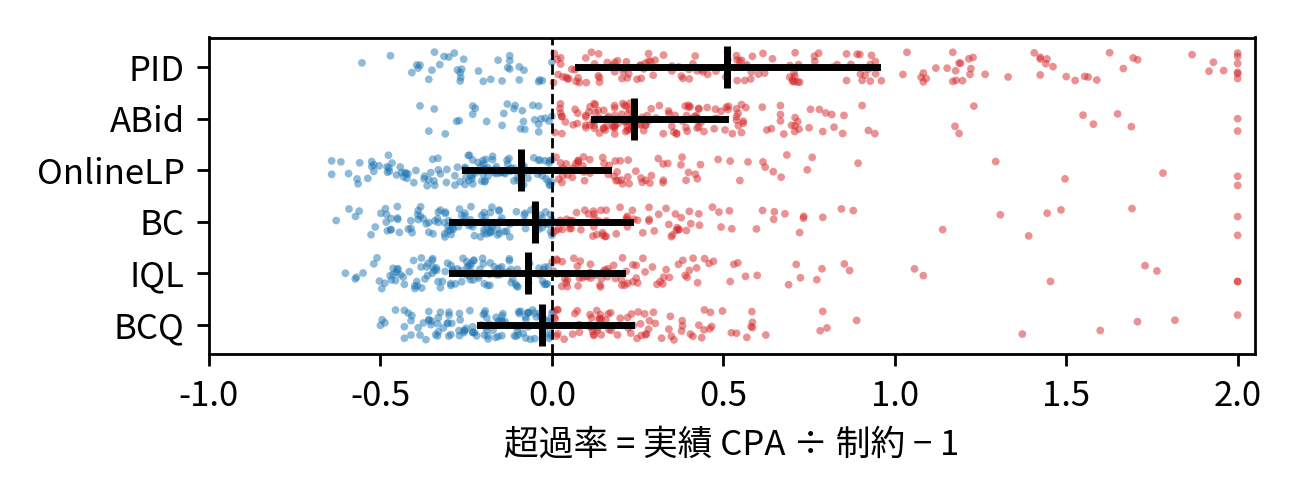
\includegraphics[width=0.74\linewidth]{fig/fig_exceedance_rate.png}
\caption{購入数が1以上のセルの超過率。黒線は25〜75\%点，縦棒は中央値（2超の点は右端）}
\label{fig:exc}
\end{figure}

1セルの購入数の中央値は，6手法とも22〜28であった。
達成条件（REP005.md）を満たし，目的は\textbf{達成}した。手法の間の差の検定はしていない。

% ============================================================
\section{結果から生まれた問い}\label{sec:e-question}
% ============================================================

落札した6手法のすべてで，0.38以上のセルが制約を超えた。超過の割合と大きさは，PID・ABidと，ほかの4手法とで違った。
制約を$\alpha$の上限に使うOnline LP（0.38）と，制約を持たないBC・IQL・BCQ（0.43〜0.45）は，近かった。

まだ確かめていないが，制約を入札に使うかどうかだけでは，この並びを説明できないと考えられる。
ABidは制約を使うのに多く，BC・IQL・BCQは使わないのに少ないためである。
また，1セルの購入数は20〜30件ほどで，購入1件の増減で実績CPAが数\%動く。
少しだけ超えたセルには，購入の抽選のぶれで超えたものが含まれている可能性がある。

既存手法の実績CPAは，どういう仕組みで制約を超えるのかを知りたい。

\end{document}
